\documentclass{scrartcl}

\usepackage[utf8]{inputenc}


% zus�tzliche mathematische Symbole, AMS=American Mathematical Society 
\usepackage{amssymb}
\usepackage{amsmath}
\usepackage{amsthm}
\usepackage{bbm}
\usepackage{color}
\usepackage{listings}
\usepackage{pdfpages}
\usepackage{csquotes}
\usepackage{float}

% f�rs Einbinden von Graphiken
\usepackage{graphicx}

% f�r Namen etc. in Kopf- oder Fu�zeile
\usepackage{fancyhdr}
\usepackage{tikz}
\usetikzlibrary{arrows, automata}

% erlaubt benutzerdefinierte Kopfzeilen 
\pagestyle{fancy}

% Definition der Kopfzeile
\lhead{
\begin{tabular}{lll}
Maciej Janowski \\
\end{tabular}
}
\chead{}
\rhead{\today{}}
\lfoot{}
\cfoot{Seite \thepage}
\rfoot{} 

\begin{document}

\section*{LAB}
\subsection*{Task}
Our task was to work a little with CNN and MNIST dataset. We had to define the structure and train the network. After that, we had to study the influence of learning rate and a number of filters on network performance. That led to the conclusion that properly chosen parameters are really important. As result, we introduced random search and studied the best performing configuration. 

\subsection*{Architecture of the network}

\begin{table}[h]
	\centering
\begin{tabular}{|c||c|c||c|}
	\hline
	\textbf{Layer} & \textbf{\# of Units} & \textbf{Activation function} & \textbf{Size} \\ \hline \hline
	Convolutional layer & 16 & ReLu & 3 \\ \hline
	Pooling layer & -  & -  & 2 \\ \hline
	Convolutional layer & 16  & ReLu & 3 \\ \hline
	Pooling layer & -  & - & 2 \\ \hline
	Dense layer & 1024  & ReLu & -  \\ \hline
	Logits layer & 10  & Sigmoid  & - \\ \hline
\end{tabular}
\caption{Parameters for each layer}
\end{table}

\subsection*{Default values}

\begin{figure}[H]
	\centering
	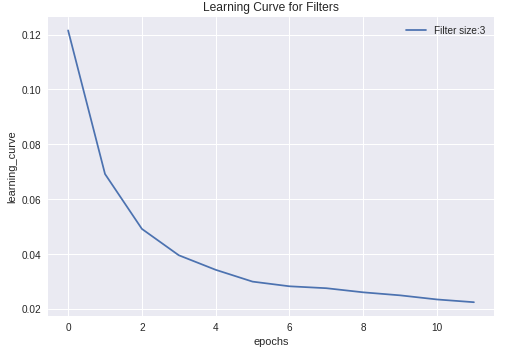
\includegraphics[scale=0.6]{1}
	\caption{Learning curve}
	\label{fig:1}
\end{figure}

\subsection*{Learning rate importance}

\begin{figure}[H]
	\centering
	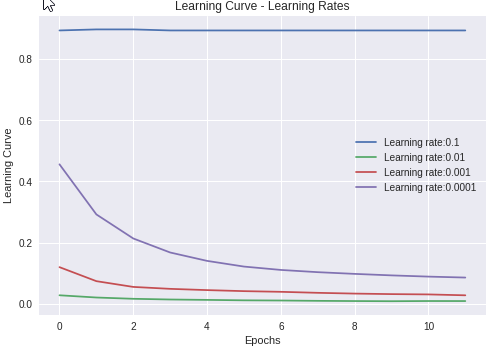
\includegraphics[scale=0.6]{2}
	\caption{Learning curve}
	\label{fig:2}
\end{figure}


\subsection*{Number of filters importance}

\begin{figure}[H]
	\centering
	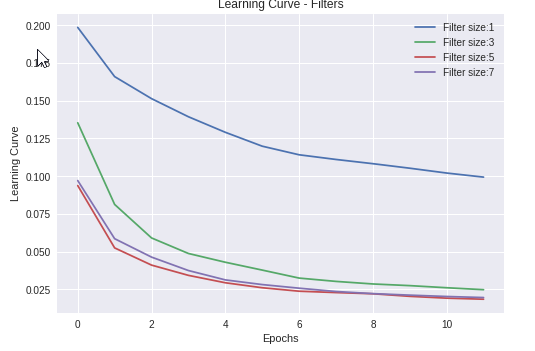
\includegraphics[scale=0.6]{3}
	\caption{Learning curve}
	\label{fig:3}
\end{figure}


\subsection*{Random search}

\begin{figure}[H]
	\centering
	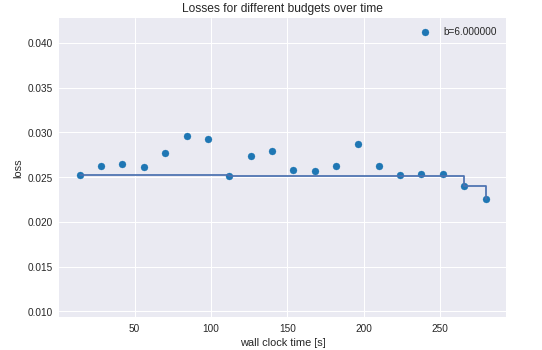
\includegraphics[scale=0.6]{4}
	\caption{Loss}
	\label{fig:4}
\end{figure}

\subsection*{Best performing configuration}

\begin{figure}[H]
	\centering
	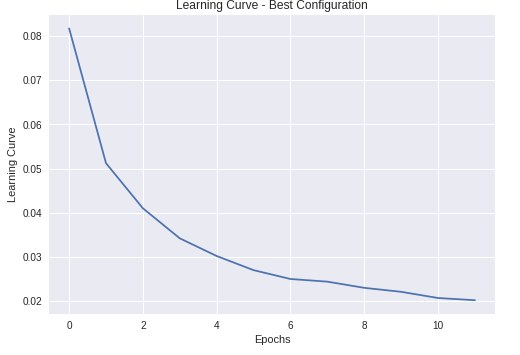
\includegraphics[scale=0.6]{5}
	\caption{Learning curve}
	\label{fig:5}
\end{figure}


\subsection*{Comments}

\begin{itemize}
	\item I got some problems running the code on my Windows-based machine, after a long fight I switched to Google Colab. I hope it is not a big inconvenience.
	\item I will provide the Google Colab notebook with the results saved in the output, I will also try to create .py files, but I cannot check if they are running properly
\end{itemize}
\end{document}


